\section{Computação Afetiva}

\citet{Pic98} definiu Computação Afetiva como uma ``computação relacionada,
surgida ou que influência as emoções''. Além disso, computadores com emoções
permitem aos mesmos um determinado nível de comportamento inteligente e
criatividade que seria impossível sem as emoções e esse é o principal desafio
dessa área. Logo, o seu entendimento pode explicar fenômenos como, por
exemplo, atenção, memória e outros.

Essa área é normalmente dividida em duas sub-áreas. A primeira estuda o
reconhecimento e a expressão de emoções dentro da IHC;
a segunda, foca na síntese de emoções para aprimorar os seres robóticos e/ou
para estudar o comportamento humano por meio de simulações. Há muita
aplicabilidade dessas técnicas, por exemplo: a área que reconhece as emoções
pode ser utilizada para adaptar o sistema ao estado da pessoa permitindo ao
mesmo instruí-la, questioná-la, encorajá-la ou ocultar informações irrelevantes.

O objetivo de \citet{bick2003relational} com o projeto \emph{Relational
Agents} é possibilitar aos usuários a criação de um relacionamento social e
emocional com longa duração.  Em \citet{bickmore2009virtual}, a confiança no
agente torna possível discutir tarefas mais importantes como melhoria da saúde
ou até a compra de uma casa. Outro trabalho na área de IHC é o reconhecimento
de emoções para aumentar a imersão em jogos, por exemplo permitindo ao próprio
jogo adaptar eventos ou trechos tornando-o mais divertido.

\begin{figure}
  \begin{center}
    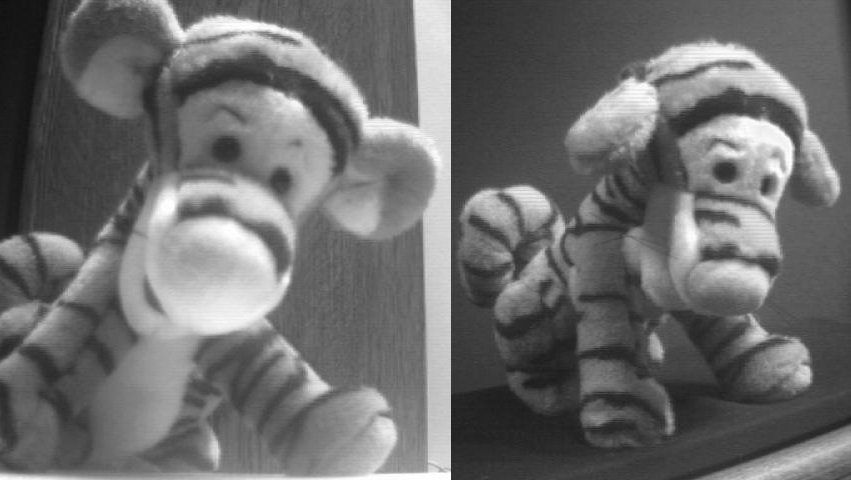
\includegraphics[width=75mm]{figuras/tigger-mit.png}
  \end{center}
  \caption{Brinquedo que responde as emoções das crianças \cite{kirsch1999affective}.}
  \label{fig:tigger-mit}
\end{figure}

O projeto \emph{The Affective Tigger: a reactive expressive toy} de
\citet{kirsch1999affective} é um brinquedo capaz de reconhecer e reagir às
emoções exibidas pelas crianças. Por exemplo, quando a criança encontra-se
feliz, o boneco expressa felicidade (ver Figura~\ref{fig:tigger-mit}). Ao todo
existem 5 estados emocionais: muito feliz, feliz, neutro, triste e muito
triste. Todos, com exceção do neutro, possuem alguma síntese vocal como um
rosnado (tristeza) ou uma risada (muito feliz). Assim, esse brinquedo, por ser
considerado um ser robótico que reage à criança com seus próprios estados
emocionais, fica enquadrado na segunda área.  Portanto, o desenvolvimento
desse brinquedo serviu para aprimorar os seres robóticos.

O projeto AIDA\footnote{Mais detalhes, ver http://senseable.mit.edu/aida} (do
inglês \emph{Affective Intelligent Driving Agent}) pode ser entendido como
enquadrado na área de IHC, pois o interesse é entender o estado afetivo da
pessoa dirigindo. Além disso, interessa-se em ter um relacionamento com o
usuário sugerindo alterações nas rotas baseando-se na rotina aprendida depois de
um tempo de aprendizado.  A pesquisa relatada em \citet{dias-agents} visou
melhorar a simulação de agentes através do uso da emoção guiando o processo
deliberativo e melhorando o entendimento e gerência das emoções.  O presente
trabalho se enquadra na área de síntese de emoção, pois o interesse é em
entender o estado emocional e como ele pode afetar o comportamento de um
personagem.

\subsection{Modelo Cognitivo Emocional} \label{ch-ca-mce}

Estudos neurológicos recentes \cite{ledoux1998emotional,damasio2004erro}
mostram a importância das emoções na tomada de decisão.
\citet{damasio2004erro} definiu emoção como sendo um estado físico do corpo
que se altera de forma contínua. Sendo assim, o sentimento foi definido como a
percepção dessas alterações.

Na psicologia há diferentes modelos que tentam explicar a afetividade.
\citet{scherer2000tnoe} categorizou esses modelos afetivos em quatro
categorias principais: modelos dimensionais, modelos discretos, modelos
baseados em significados e modelos baseados em componentes. A primeira
categoria visa descobrir variáveis que representam eixos das classes emotivas
e estabelecem meios de se mover por esses eixos. A seguinte, especifica um
conjunto básico de emoções e regras de evolução para esse conjunto.
Já, a categoria dos baseados em significados se preocupa com as situações
em que o sentimento foi ocasionado e tenta descrever as estruturas semânticas dos
mesmos. A última, entende que os sentimentos são aprendidos ao longo do tempo.
Sendo assim, os modelos baseados em componentes estudam o elo entre os
sentimentos e as suas situações. Esse elo é montado de diferentes formas e
varia de pessoa para pessoa.

\begin{figure}[t]
  \centering
    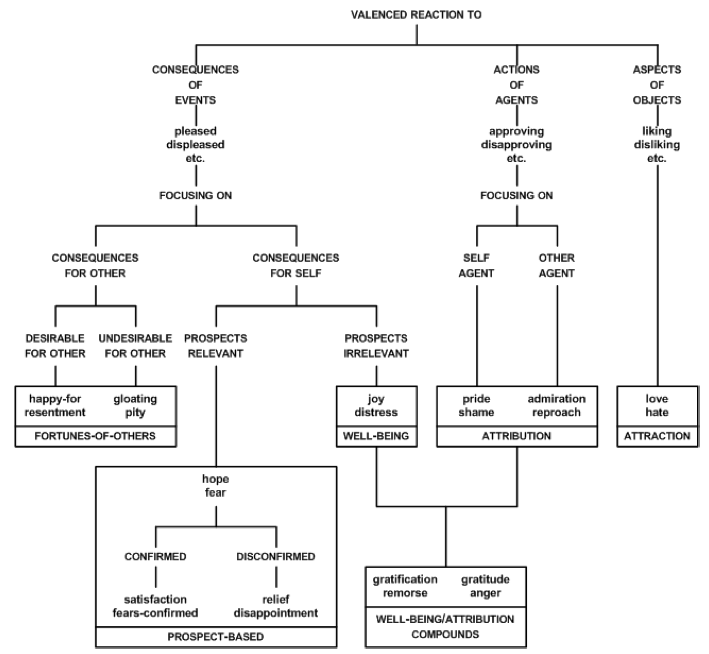
\includegraphics[width=150mm]{figuras/occ.png}
  \caption{Estrutura de emoções \cite{ortony1988cse}.}
  \label{fig:occ_model}
\end{figure}

Um modelo baseado em significados, bastante conhecido na Inteligência
Artificial, foi definido por \citet{ortony1988cse}. Nesse modelo\footnote{A
partir daqui o modelo será referenciado como modelo \emph{OCC}.} são descritos
22 emoções com suas situações. Essas emoções são divididas em formas de se
perceber o mundo a sua volta por consequências (importância das metas),
ações (julga a responsabilidade) e objetos (atração ou repulsa). Assim sendo,
essas maneiras de se perceber o mundo refletem diferentes jeitos de se
analisar as situações que podem ser relativas aos objetivos, valores morais ou
gostos da pessoa.

A Figura~\ref{fig:occ_model} resume esse modelo e mostra as
percepções possíveis de um indivíduo.  Partindo da direita para esquerda, o
ramo mais básico, \emph{Aspects Of Objects}, é ativado quando se avalia o
gosto de alguém para algum objeto (inanimado ou não). Por exemplo, Millie
gosta de rosas azuis. No seguinte, \emph{Actions Of Agents}, o julgamento das
ações exercidas por outro indivíduo ou por si mesmo é baseado nos
valores morais da pessoa que está julgando. Exemplo: reprovar a atitude dos
bancários que fazem greve a cada ano. Cabe salientar, que ao julgar ações, o
modelo permite um grau de ``empatia'' chamado pelos autores de ``unidade de
força cognitiva''\footnote{Traduzido literalmente de \emph{Strength of
cognitive unit}.}. Dessa forma, é possível, por exemplo, ficar com orgulho
porque uma atleta ganhou uma medalha ou ficar envergonhado ao descobrir que o
vizinho bate no(s) filho(s).

O último ramo da árvore, mais a esquerda na Figura~\ref{fig:occ_model}, é o
\emph{Consequences Of Events} que representa as coisas que aconteceram (e
foram consideradas importantes), acontecem ou acontecerão (objetivos
almejados)\dev{}. Essas emoções são avaliadas segundo as suas consequências
para o alcance ou impedimento dos seus objetivos. Exemplos possíveis desse
ramo do modelo são a emoção sentida ao receber uma boa nota em um teste, ao
ser assaltado ou ao perceber não ser possível chegar em um destino planejado.

Todas as emoções do modelo trabalham com duas intensidades. A intensidade da
emoção que representa o físico e a intensidade do sentimento que representa o
quanto o agente esta percebendo daquela emoção. Dessa forma, um indivíduo só
possui sentimento quando a intensidade da emoção ultrapassa um
determinado limite\dev{}.  Essa intensidade é obtida por uma função matemática
que utiliza variáveis de dois tipos: locais, que influenciam as emoções do ramo
específico; e globais, que influênciam todas as emoções do modelo.  Um exemplo
de variável local é o desejo, enquanto um exemplo de variável global pode ser
o senso de realidade de uma pessoa.

\citet{bates1994role} foi um dos primeiros a trabalhar na utilização de emoções
na área de animação. Nessa área, o estudo do comportamento humano é realizado
visando imitar as ações humanas. Assim, a principal afirmativa do trabalho era
que o comportamento emotivo de um personagem é um papel importante para que o
mesmo pareça ter vida própria. Dessa forma, esse trabalho utilizou o modelo
descrito visando melhorar a credibilidade de seus atores. Por exemplo, um dos
agentes lida com o medo sendo agressivo com os outros enquanto outro agente
lida com a mesma emoção sendo retraído.

%% Comentado mas iria em trabalhos relacionados...
%\citet{GraCli98} criaram um mecanismo evolucionário utilizando redes neurais
%com uma base química para guiar o comportamento do ator. Os atores simulados
%podem envelhecer, aprender e, inclusive, se reproduzir (aqui são utilizados
%algoritmos genéticos).  Por exemplo, o personagem pode aprender algumas
%palavras básicas e demostrar que esta envelhecendo por meio da mudança da cor
%de seus cabelos dando uma certa ilusão de vida.

Visando entender melhor o impacto da emoção na tomada de decisão,
\citet{zhang2009emotional} desenvolveram uma aplicação que os sentimentos
afetam o planejamento das ações à serem realizadas.
\citet{neto2010construction} focaram no mesmo objetivo, porém visando estudar
o impacto da memória no planejamento. Sendo assim, um meio para o agente
``esquecer'' determinadas crenças quando o estado emocional for diferente
daquele guardado anteriormente foi feito. Essa característica torna o
planejamento e as atitudes dos personagens virtuais mais realista.

Um dos trabalhos mais conhecidos baseado no modelo \occ é, sem dúvida, o de
\citet{kshirsagar2002multilayer}. Ele utilizou
as emoções levantadas no modelo em conjunto com um modelo de personalidade
baseado na psicologia que leva em consideração 5 fatores: extroversão,
agradabilidade, conscientização, neurose e receptividade. O primeiro, descreve
a preferência para o comportamento em situações sociais. O seguinte, a
interação com os outros indivíduos. A conscientização é a organização e
persistência das metas. A tendência de pensamentos negativos é a neurose ou
fator neurótico. Por fim, o último, descreve se a pessoa tem interesse em
cultura ou é ``cabeça aberta'' para novas ideias.

\subsection{Ontologias Afetivas}

De acordo com \citet{Gutierrez:2007:OVH:1229160.1229164}, uma
ontologia possui inúmeras utilidades tanto em pesquisa quanto na
indústria. Na pesquisa o foco é uma melhor descrição do domínio propriamente
dito, enquanto na indústria o foco é a melhor utilização dos recursos de seus
colaboradores. As ontologias emocionais visam descrever emoções ou aspectos
afetivos de um indivíduo se baseando ou não em estudos da psicologia.

Em \citet{benta2007ontology} foi feita a construção de uma ontologia escrita em
\emph{OWL}. Nesse trabalho as emoções são divididas em primárias e secundárias, as
secundárias se originam a partir das primárias. As emoções primárias,
não cognitivas, são: \emph{Angry}, \emph{Disgust}, \emph{Fear},
\emph{Happy}, \emph{Neutral}, \emph{Sad} e \emph{Surprise}. As emoções
secundárias, cognitivas, descritas são ao todo 4. O interessante aqui é que
essas 4 emoções são inferidas a partir de relações entre os objeto. Além disso,
há o conceito de emoção ativa que é a emoção predominante naquele momento. O
valor da emoção é calculado da seguinte forma, a sensibilidade (predisposição
a emoção varia de 0 à 1) multiplicado pela intensidade da emoção. A emoção
predominante é o maior valor entre as emoções.

No modelo \occ a distinção entre os tipos de
emoções não existe porque se pressupõe que toda emoção exige um certo nível de
cognição. Não existem, também, um limite no que pode ou não ser percebido em
quantidade de emoções. Mas, existe um limite de perseguir uma meta por vez.
Fora isso, se pode pensar que emoções opostas compartilham os mesmos atributos
e, por isso, essas emoções não serão sentidas ao mesmo tempo.

Não tendo nenhuma informação de uma teoria de emoções específicas modeladas em
sua ontologia, \citet{wks2008towards} criaram uma ontologia de alto nível se
aproveitando de outra ontologia de alto nível e de uma de analise léxica.
Assim, o principal conceito desse trabalho é o de sensor que é um objeto
físico no ambiente e que recebe as informações do meio e as ``transportam''
para o mundo mental do agente. Sendo assim, é possível reconhecer a
percepções similares e descrever novas situações. Todavia, o presente trabalho
não tem objetivo de criar uma ontologia de alto nível\dev{}.

\citet{springerlink:10.1007/978-3-642-01639-448} desenvolveram um motor de
emoções que utiliza um modelo de mistura de emoções em conjunto com o modelo
\emph{OCC}. O trabalho deles utilizou o conceito de camadas onde cada camada tem uma
responsabilidade distinta e que visa complementar a anterior. Essas são ao todo
quatro: classificação, interação, mapeamento e expressão. A primeira visa
determinar que categoria ou ramo será afetado. A seguinte, determina a
intensidade da emoção. A de interação analisa os efeitos nas categorias
emocionais do personagem. A próxima, mapeia as 22 emoções do modelo para pelo
menos uma expressão. A expressão propriamente dita é feita pela camada de
expressão.

Esse trabalho ainda utilizou um modelo dimensional para misturar as emoções
primárias. Assim, as emoções secundárias podem ser descobertas a partir do
nível dos eixos afetados. O trabalho mostra quase todas as emoções do
ramo de consequência de eventos, com exceção das emoções de \emph{Hope} e
\emph{Fear}. As emoções primárias são as emoções do modelo \occ e como
secundárias estão as emoções construídas a partir da mistura dessas emoções.
Essa diferenciação, como dito anteriormente, não existe no modelo \occ.

Um modelo genérico que representa o ambiente e eventos que estão envolta de um
personagem, sua personalidade e suas preferências foi feito por
\citet{lera2009semantic}. Nesse trabalho o foco eram emoções que podem ser
representadas no rosto. Assim, a identificação do contexto é feita através de
eventos e do retorno afetivo. Fora isso, as expressões faciais são modificadas
dependendo dos eventos do ambiente e, também, da personalidade, metas e
preferências dos atores virtuais.

\citet{adam2009alfototoe} formalizaram o modelo \occ de maneira lógica.
Esse trabalho descreve a probabilidade de maneira comparativa, isto é, o
evento A é mais provável que o evento B. Além disso, ha uma ordem temporal nas
ações sendo desempenhadas. O autor propõem uma diferenciação entre ação e
evento interessante. O primeiro é causado intencionalmente pelo agente\dev{},
enquanto o segundo o agente não tem controle da ação. Por exemplo, ir para
aula é uma ação e espirrar é um evento.

\subsection{Arquiteturas Emocionais} % sao so as similares (usam o OCC)

\todo {redigir}

{O Raciocinador Afetivo} % June 1992
% At least 2 pages
\cite{elliott1992tar}

{Conjunto de Ferramentas Em} % May 1996 bates-based
% At least 2 pages

{Émile}
\cite{gratch2000empitae}
A meta desse trabalho é apresentar o aplicativo chamado Émile. O modelo
permite agentes avaliarem o significado emocional de eventos deles se
relacionando com os planos e metas, modelando e predizendo os estados afetivos
de outros agentes e alterando o comportamento de acordo.  O trabalho se baseia
na ``construal theory'' (nao traduzi porque nas ciencias eh normal ter
traducoes estranhas...) que tenta estimar a relação etre eventos e a
disposição (descrita pelas metas, padrões sociais e preferencias) do agente
atraves de um conjunto de conhecimento chamado ``construal frames''. Esses
``frames'' possuem duas tarefas. Eles servem para determinar a existencia de
relações e se existirem eles caracterizam a relacao em termos de um conjunto
de caracteristicas chamadas condições emoção-elicitação.
%
O trabalho usa somente cinco emoções para ser simples: esperança, alegria,
medo, sofrimento e raiva (ou brabo). Além disso, na presente implementação o
aprendizado esta restrito as atividades de outros agentes pelas suas ações ou
por eventos comunicados (ex.: at(pier, waves).).


{EMA} % P? 2004
\cite{gratch2004domain}
O foco do trabalho é a integração de processos de raciocinadores simbolicos
como planejar, agir, comunição em linguagem natural e modelagem do usuário em
um único sistema e o papel do processamento da emoção serve para tudo isso. O
processo criado foi baseado em dois processos simples: avaliação (relacionado
com o ambiente) e imitação (que sugere estrategias de ações a serem tomadas).
As avaliações são baseadas em `variaveis de avaliação' (componentes de
avaliação ou dimensões de avaliação são outros nomes). O autor identificou as
que mais aparecem nos trabalhos e se baseou nessas para criar seu sistema
chamado EMA (EMotion and Adaptation).
%
Além disso, as estrategias de imitação podem ser baseadas no problema ou
emocional. As baseadas no problema, normalmente, possuem alguma ação envolvida
e foram encontradas 3 estrategias (copia ativa [tenta fazer], procurar suporte
social [procurar informação, conselheiro, etc] e planejar). O foco emocional
tem ao todo 11 estrategias encontradas, elas se baseam em muitas vezes rever
as prioridades anteriormente classificadas para melhorar o entendimento do
mundo. Por exemplo, é possivel aceitar uma falha, negar o que esta
acontecendo, procurar uma interpretação positiva ou, até mesmo, fazer uma
outra atividade para evitar fazer o que é necessario (mental disengagement.
Nota: No portugues isso seria procastinar! hehehehe).  Cada uma dessas
estrategias são bem explicadas juntamente com exemplo de como o processo de
imitação acontece em 5 estagios (identificação de oportunidade, elaboração da
situação, proposição de alternativas, estimativa do potencial de imitação e
seleção da estrategia). O trabalho se baseia no trabalho de Elliot (1992 -
affective reasoner) que é baseado no OCC. Uma das coisas interessantes aqui é
que são usados conceitos de frames quando esta sendo feita a avaliação, além
disso o agente mantem uma relação do que aconteceu no passado, o que esta
acotecendo e do futuro. O mecanismo de avaliação permite criar avaliações
contraditorias ou com multiplos entendimentos do mundo, entretanto para o
mecanismo de criação de avaliação não sair (enloquecido) criando avaliações
foi usado um threshold que quando atingindo é considerado um evento importante
e que merece ser avaliado, similar à idéia de ter sua atenção focada.

Eu acredito que esse trabalho eh uma estensão do que foi iniciado em 2000 pelo
Gratch.

{ALMA} %K? 2005
...

{FATIMA/fearNot!}
\cite{dias2005feeling}
O trabalho utiliza o sistema FearNot que foi desenvolvido para reduzir os
problemas de bullying nas escolas. As crianças são expostas a cenas de
bullying e fazem o papel do amigo imaginario da vitima que pode sugerir formas
de ação para situações parecidas. A arquitetura criada foi pensanda tendo em
mente: ter capacidades reativas e cognitivas, gerar credibilidade e empatia,
possuir interação com o usuário (note que os agentes não seguem cegamnte o que
o usuario diz porque isso baixaria a credibilidade) e ser independente de
dominio.
%
O autor cita Thomas and Johnston (Wall Disney) que falam que revelar os
sentimentos dos personagens também revela sua personalidade. Eles também
definem três requisitos para o sucesso da expressão emocional: deve ser
percebido sem nenhuma dúvida pela plateia; emoções podem ser acentuadas ou
exageradas para um melhor entendimento;  emoções afeitam o processo de
deliberação e consequencias devem ser notadas nas ações dos personagens.
%
O processo de deliberação do agente é focado na avaliação feita a partir do
que se percebe do ambiente em niveis reativos e deliberativos (emoções com
probabilidade). Apos o estado emocional é gerado e a memoria atualizada
paralelamente. O processo de imitação pode ser também no nivel reativo
(tendencias de ações) ou deliverativo (foco no problema ou emoção). Quando o
nivel deliverativo procede, uma reavaliação pode ser feita que afeta o estado
emocional (NOTA: caminho do cortex?) ou o entendimento do conhecimento
(memorias: modelo do mundo, metas, intencoes e planos).

{WASABI} % March? 2008
% At least 2 pages



%%???
\cite{grimaldo2006ontology}
\cite{kshirsagar2002multilayer}
